\section{}
A wood cantilever beam with cross section as shown in Fig. \ref{fig:Q1ProblemDiagram} is subjected to an inclined load P
at its free end. Determine, (a) the orientation of the neutral axis, (b) the maximum bending stress. Given
$P = 1$ kN, $\alpha = 30^{\circ}$, $b =80$ mm, $h = 150$ mm, $L = 1.2$ m.

\begin{figure}[h]
    \centering
    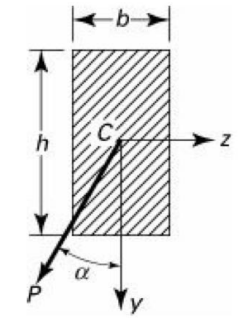
\includegraphics[width=0.3\textwidth]{Questions/Figures/Q1ProblemDiagram.png}
    \caption{Problem Diagram}
    \label{fig:Q1ProblemDiagram}
\end{figure}

Finding the moments, 
\begin{align*}
    M_y &= -P L \sin(\alpha) = 1 \times 1.2 \times \sin(30^{\circ}) = -0.6 \text{ kNm}\\
    M_z &= P L \cos(\alpha) = 1 \times 1.2 \times \cos(30^{\circ}) = 1.04 \text{ kNm}
\end{align*}

Moment of inertias
\begin{align*}
    I_y &= \frac{1}{12} b^3 h = \frac{1}{12} \times 80^3 \times 150 = 6.4 \times 10^6 \text{ mm}^4\\
    I_z &= \frac{1}{12} h^3 b = \frac{1}{12} \times 150^3 \times 80 = 2.25 \times 10^7 \text{ mm}^4
\end{align*}
Since the $y$ and $z$ axes are axes of symmetry, $I_{yz} = 0$.

The neutral axis is given by
\begin{align*}
    \tan{\phi} &= \frac{M_y I_z}{M_z I_y} \\
    &= \frac{-0.6 \times 10^6 \times 2.25 \times 10^7}{1.04 \times 10^6 \times 6.4 \times 10^6} \\
    &= -2.03 \\
    \implies \phi &= \arctan(-2.03) = \boxed{-63.77^{\circ}}
\end{align*}

\subsection{}
The maximum bending stress is at the furthest point from the neutral axis, which is at the top left 
or bottom right corner of the cross section. Using the bottom right point,
\begin{align*}
    \sigma_{x}  &= \frac{M_{y'} z'}{I_y} - \frac{M_{z'} y'}{I_z} \\ 
    &= \frac{-0.6 \times 10^6 \times 80/2}{6.4 \times 10^6} - \frac{1.04 \times 10^6 \times 150/2}{2.25 \times 10^7} \\
    &= \boxed{-7.22 \text{ MPa}}
\end{align*}